\section{Implementation}

\subsection{Solution Strategy}
\subsubsection{Architecture decisions}
\par Our project is based on REST architecture. It consists of client and web server parts. Without much detail, our clients send a request to the server (like GET and POST HTTP requests), and depending on conditions server-side gives a response. For example, the client wants to see some protected page, for example, the client sends a request to the webserver. If the request is valid (for instance, the user is logged in), then we give him access to this part of the info. It is worth mentioning, that the main advantage of REST architecture is in task separation. Generally, all related to UI and Backend is separated into two parts, and interaction is done via JSON or something like XML. Besides, it makes code less chaotic and also more secure. 
\subsubsection{Technology stack}
\par After a long consideration, we decided to use the next technology stack:  
\begin{enumerate}
\item html/CSS + React (frontend);  

\item Python with flask framework (backend); 

\item Nginx + Gunicorn + dokku + drone.io (Nginx - proxy for frontend and gunicorn backend, gunicorn - python wsgi server, dokku - deployment, drone.io - continuous integration)  

\item Gitea (similar to GitHub) this is like architecture decision + technology stack 
\end{enumerate}


\subsection{Project initialization}
\subsubsection{Task management/distribution}
\par As management tool we choose to use notion.so - mainly because it offers students a pro version, as well as allow us to use the Notion platform as a common blackboard, to-do list and to keep easy track of what everyone has done or what is supposed to do next.
Below is a snapshot of our notion dashboard:
\par 

\includegraphics{Notio_Logo.png}
\par
\begin{figure}[!h]

	
	
	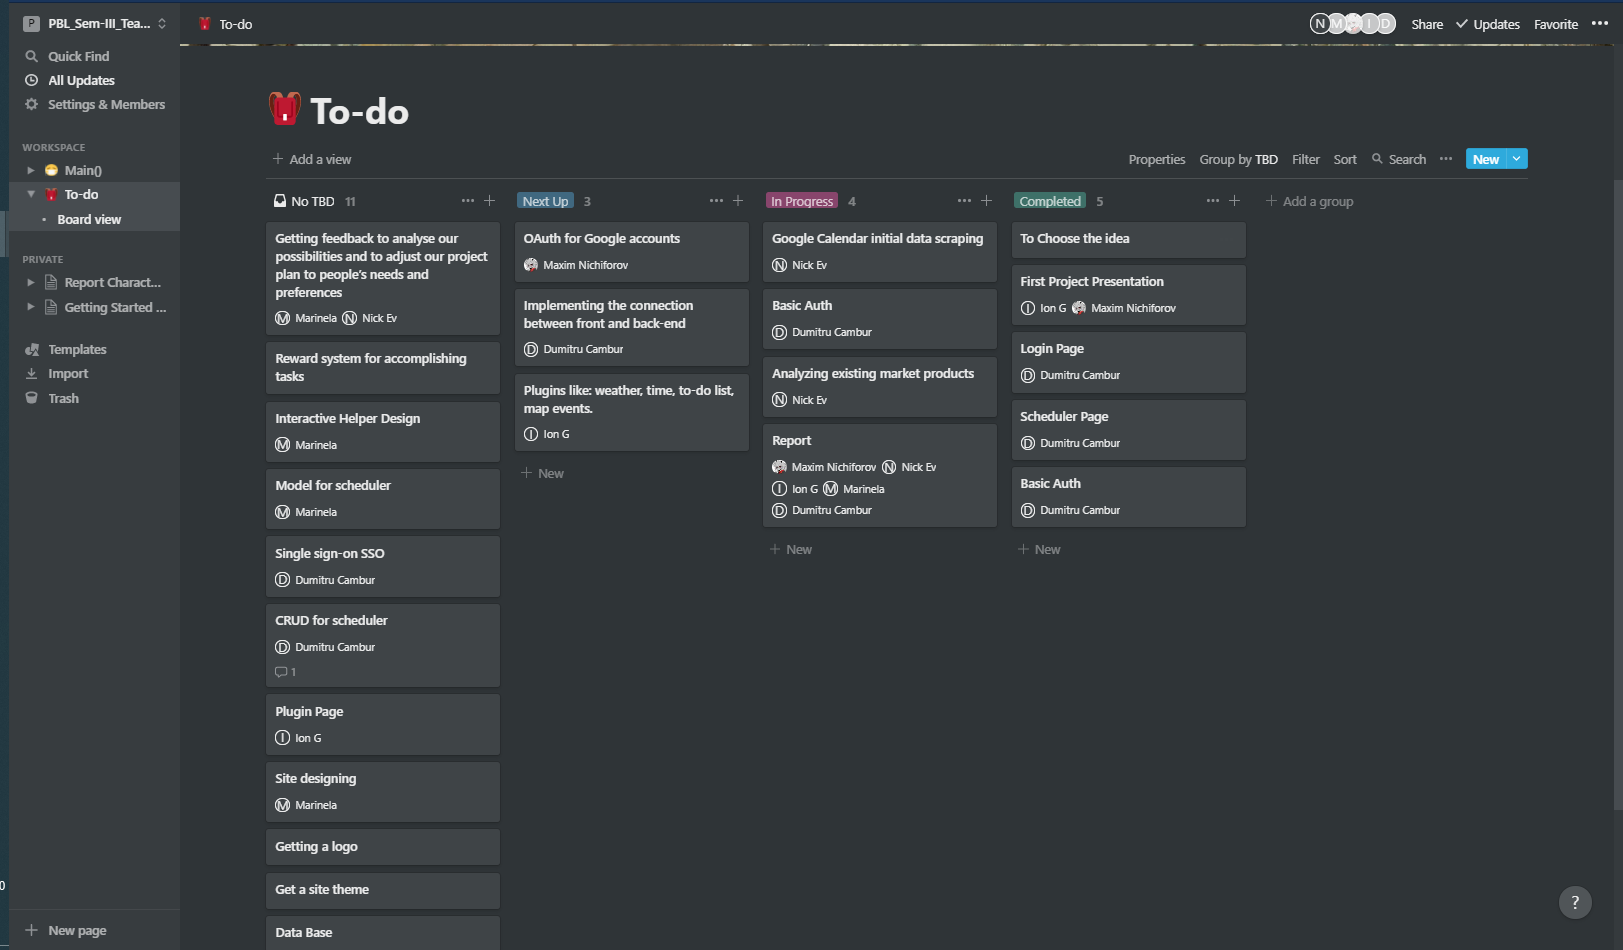
\includegraphics[width=\textwidth]{TaskManagment1}
	
	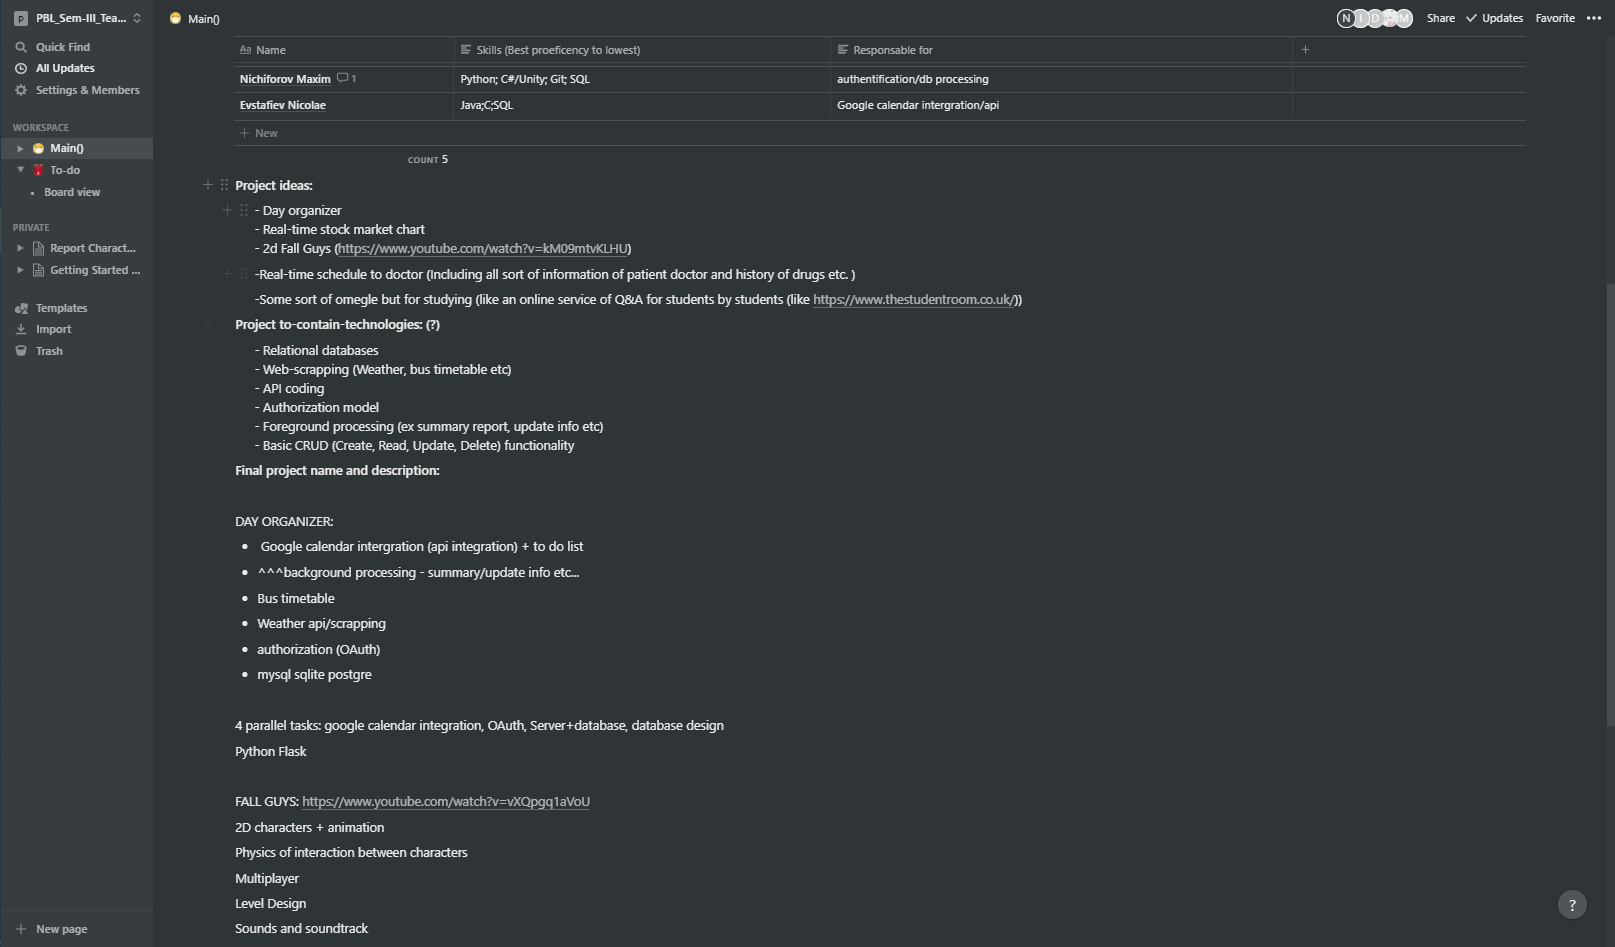
\includegraphics[width=\textwidth]{TaskManagment2}
	\caption {Notion platform used to share tasks}
\end{figure}


\subsubsection{Distributed Version Control of the involved repositories}
\par We choose to use Git and to host our code base on Gitea over GitHub, as it offers better overall features that we may need in future upon developing further the project. 
Gitea is an open-source forge software package for hosting software development version control using Git as well as other collaborative features like bug tracking, wikis and code review. It supports self-hosting but also provides a free public first-party instance hosted on DiDi's cloud.
Source code hosted on Gitea:\\
 Front-end part:\url{https://git.bitcore.nz/dima/day_organizer_fe}\\
 Back-end part: \url{https://git.bitcore.nz/dima/DayOrganizer-be}\\
 Initial work done on GitHub (no longer maintained):\url{ https://github.com/waffle4everyone/PBL_Organizer	}
 \subsection{Screenshots}
 \par
 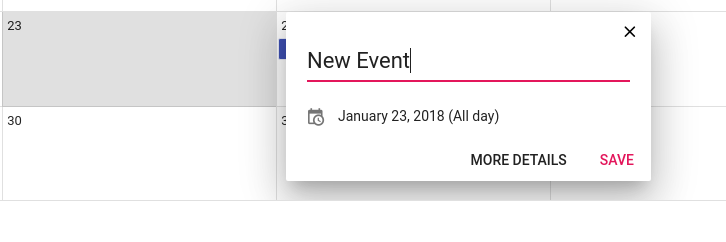
\includegraphics[width=\textwidth]{Event}
 \par
 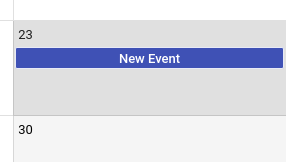
\includegraphics[width=\textwidth]{event2}
 \par
 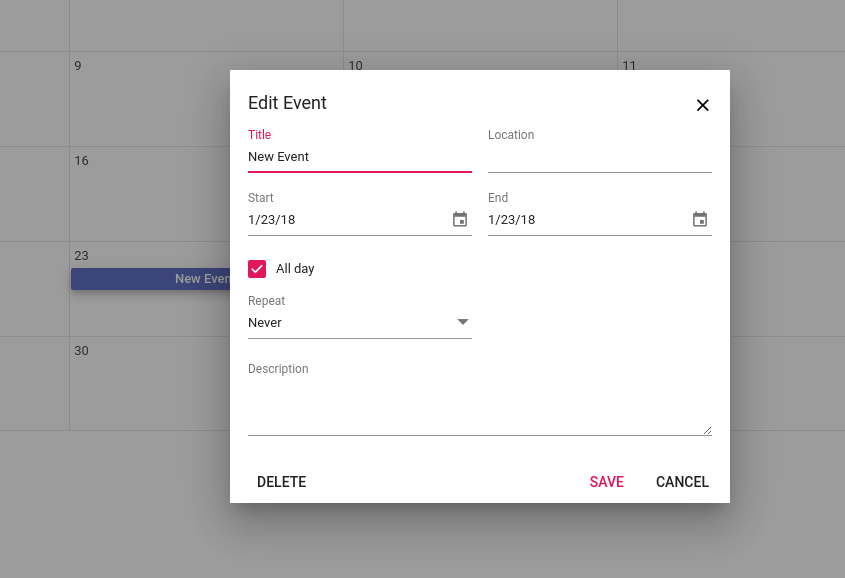
\includegraphics[width=\textwidth]{editevent}
 \par
 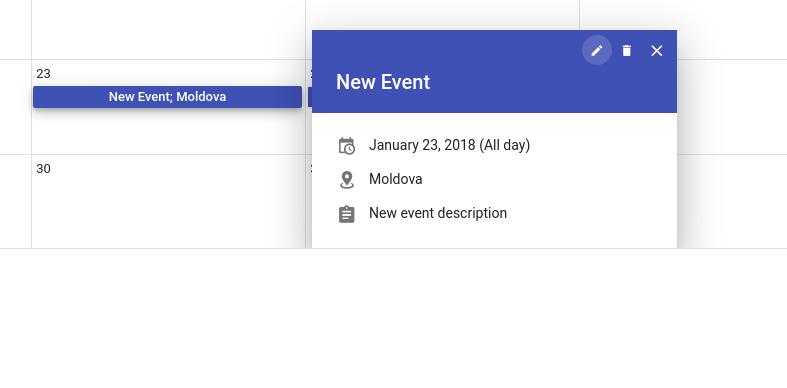
\includegraphics[width=\textwidth]{new event}
 \par
 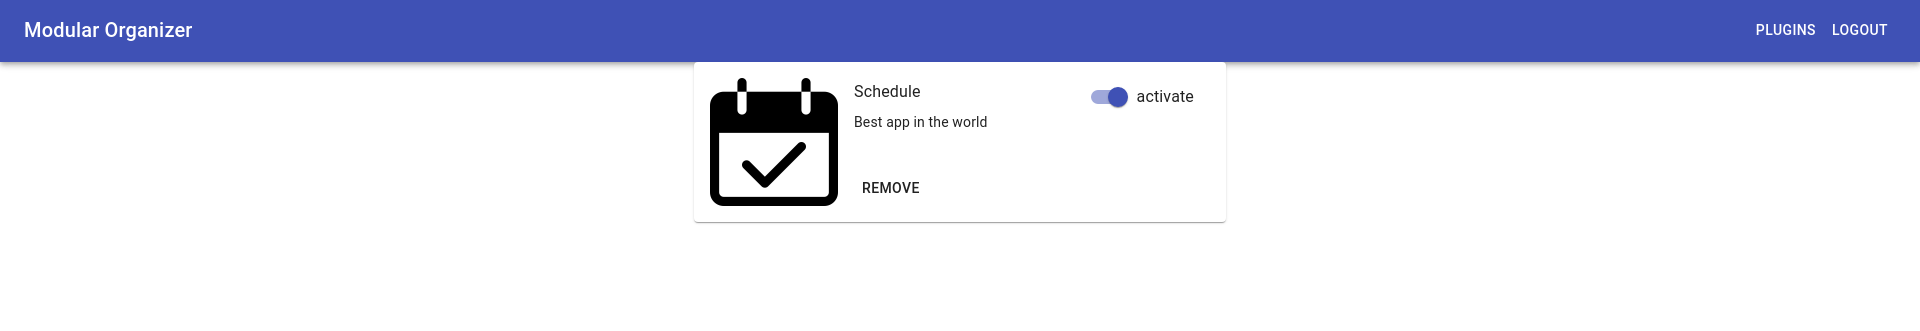
\includegraphics[width=\textwidth]{schedule}
 \par
 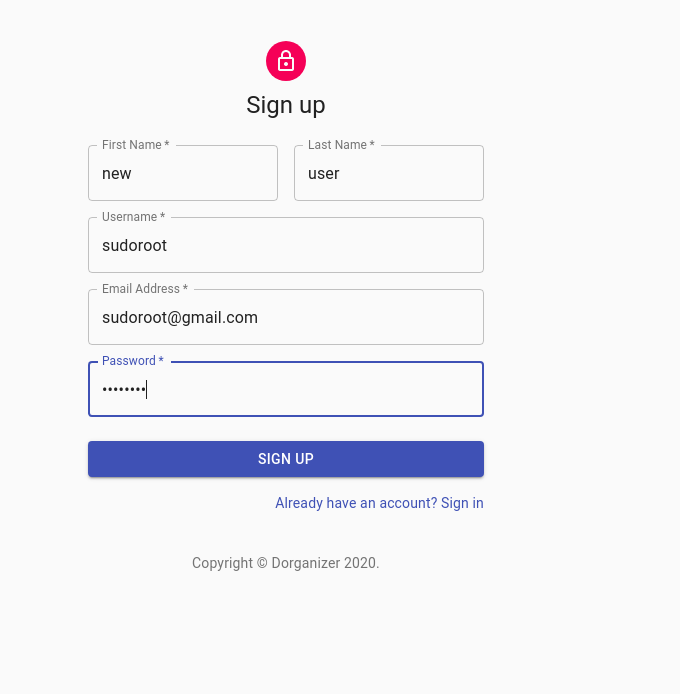
\includegraphics[width=\textwidth]{singup}
 \par
 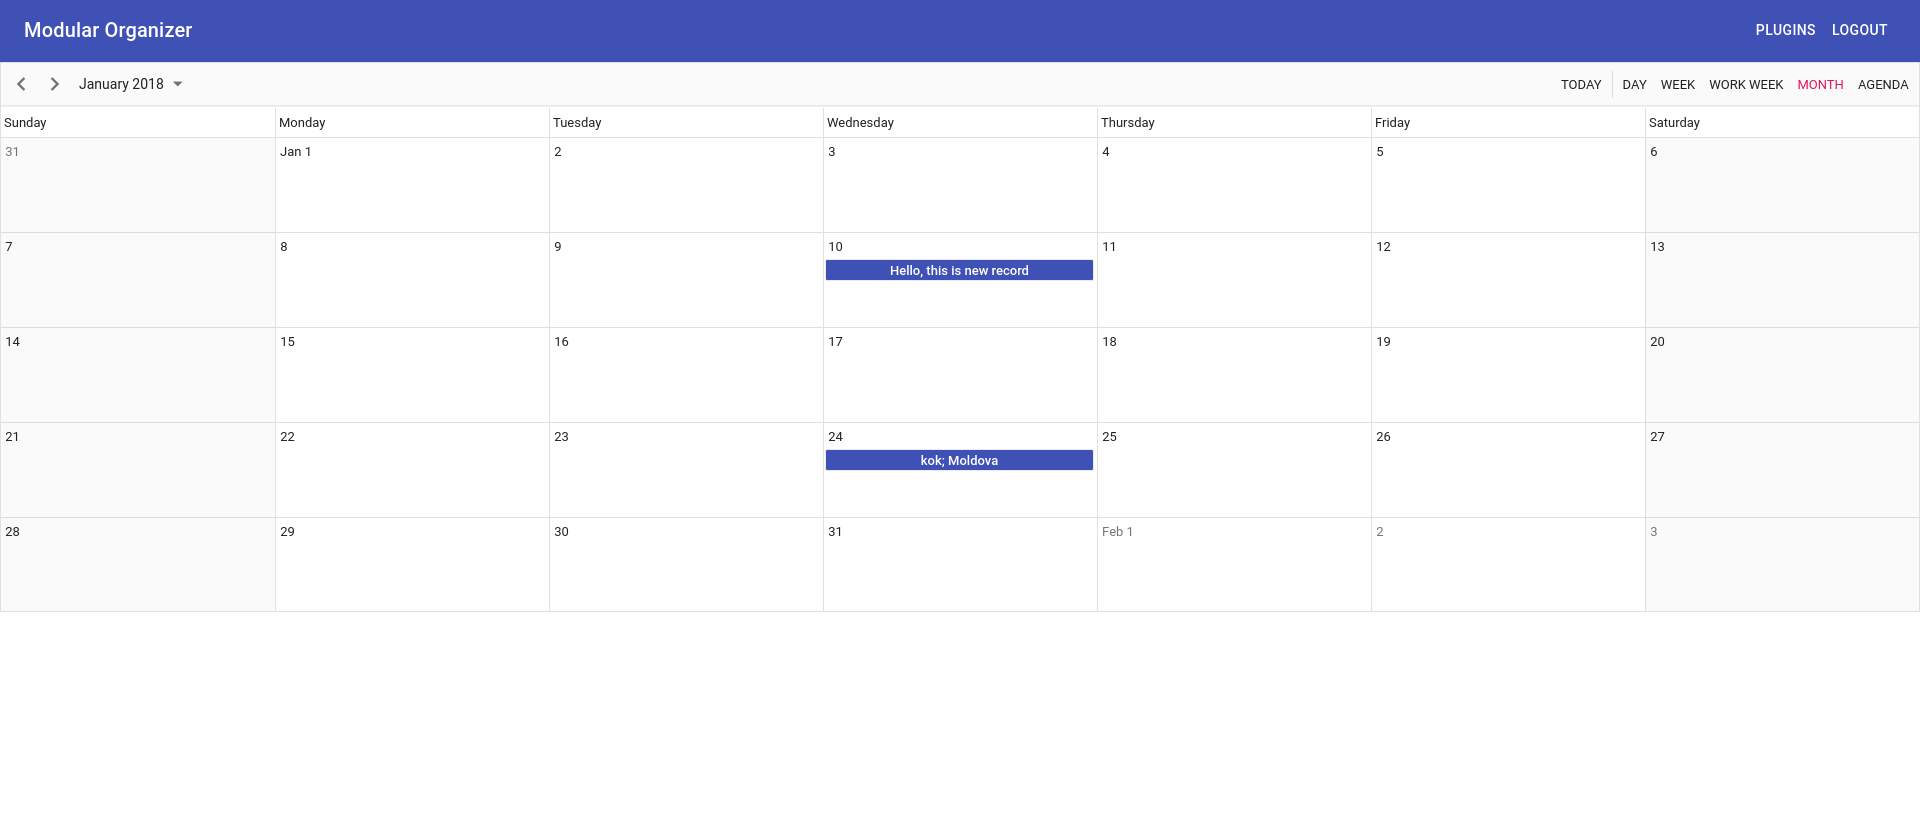
\includegraphics[width=\textwidth]{Calendarpng}
 \par
 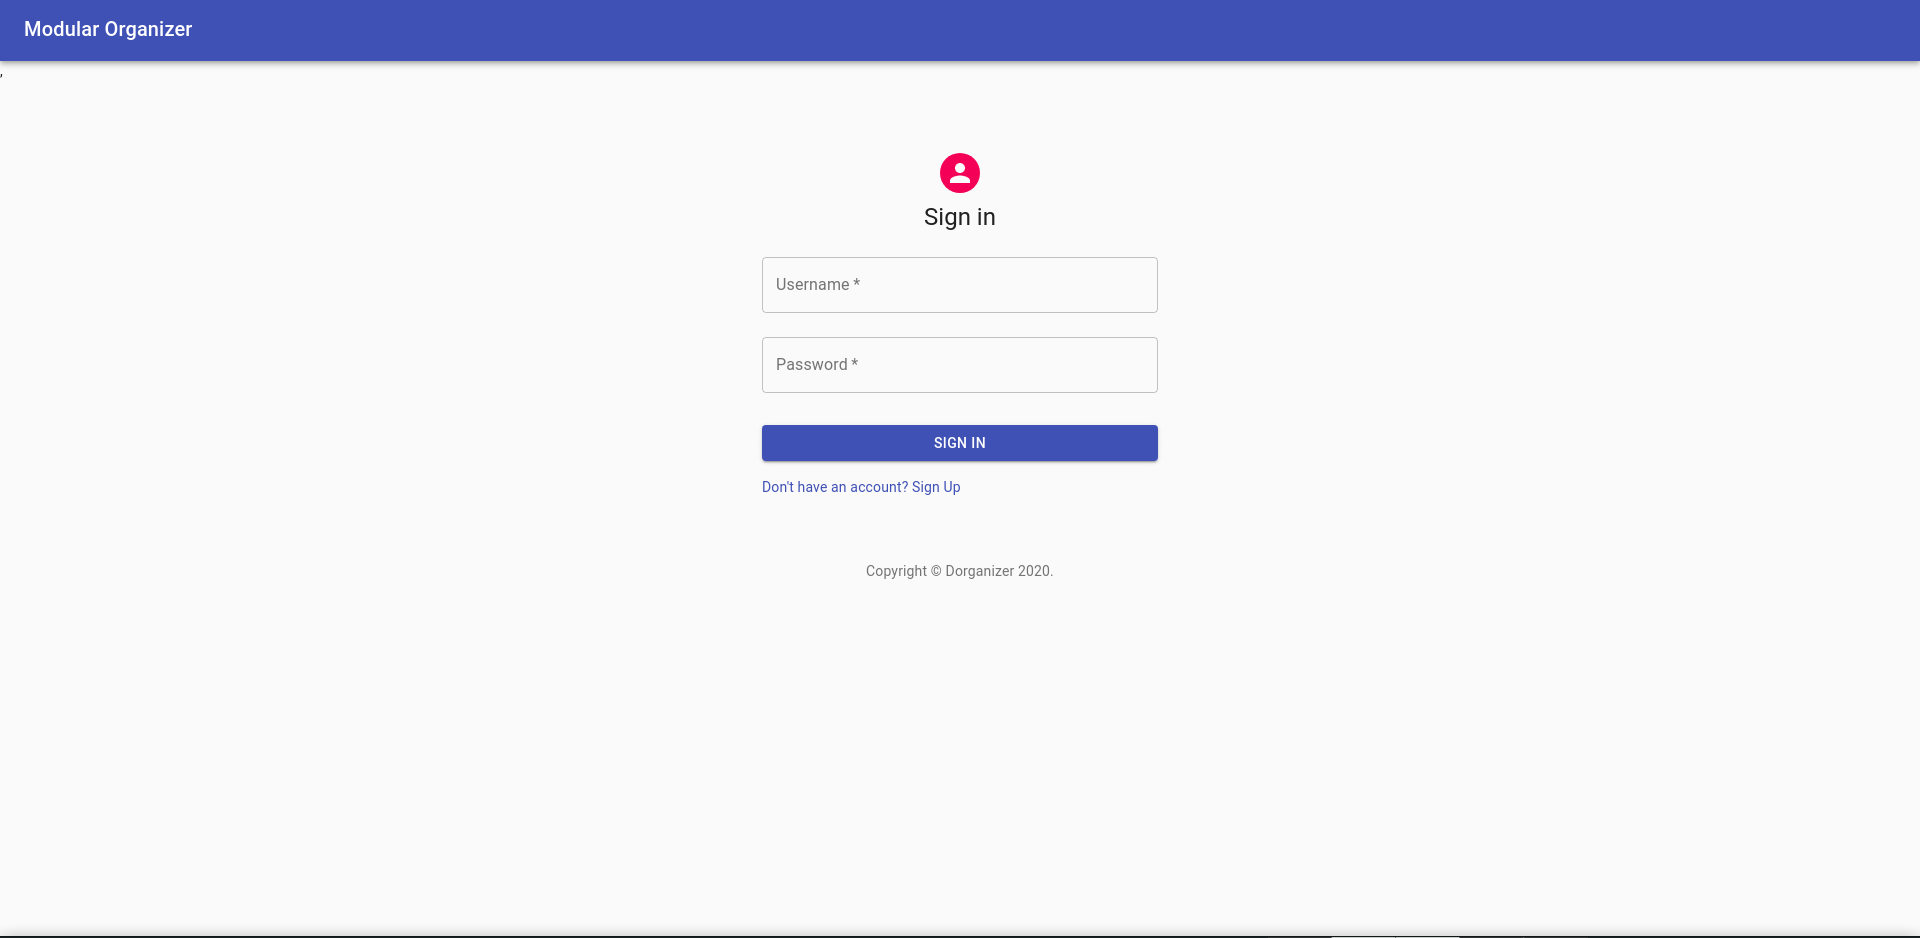
\includegraphics[width=\textwidth]{LoginPage}
 


\clearpage